\documentclass[letterpaper,12pt]{article}

\usepackage{threeparttable}
\usepackage{geometry}
\geometry{letterpaper,tmargin=1in,bmargin=1in,lmargin=1.25in,rmargin=1.25in}
\usepackage[format=hang,font=normalsize,labelfont=bf]{caption}
\usepackage{amsmath}
\usepackage{mathrsfs}
\usepackage{multirow}
\usepackage{array}
\usepackage{delarray}
\usepackage{listings}
\usepackage{amssymb}
\usepackage{amsthm}
\usepackage{lscape}
\usepackage{natbib}
\usepackage{setspace}
\usepackage{float,color}
\usepackage[pdftex]{graphicx}
\usepackage{pdfsync}
\usepackage{verbatim}
\usepackage{placeins}
\usepackage{geometry}
\usepackage{pdflscape}
\synctex=1
\usepackage{hyperref}
\hypersetup{colorlinks,linkcolor=red,urlcolor=blue,citecolor=red}
\usepackage{bm}


\theoremstyle{definition}
\newtheorem{theorem}{Theorem}
\newtheorem{acknowledgement}[theorem]{Acknowledgement}
\newtheorem{algorithm}[theorem]{Algorithm}
\newtheorem{axiom}[theorem]{Axiom}
\newtheorem{case}[theorem]{Case}
\newtheorem{claim}[theorem]{Claim}
\newtheorem{conclusion}[theorem]{Conclusion}
\newtheorem{condition}[theorem]{Condition}
\newtheorem{conjecture}[theorem]{Conjecture}
\newtheorem{corollary}[theorem]{Corollary}
\newtheorem{criterion}[theorem]{Criterion}
\newtheorem{definition}{Definition} % Number definitions on their own
\newtheorem{derivation}{Derivation} % Number derivations on their own
\newtheorem{example}[theorem]{Example}
\newtheorem{exercise}[theorem]{Exercise}
\newtheorem{lemma}[theorem]{Lemma}
\newtheorem{notation}[theorem]{Notation}
\newtheorem{problem}[theorem]{Problem}
\newtheorem{proposition}{Proposition} % Number propositions on their own
\newtheorem{remark}[theorem]{Remark}
\newtheorem{solution}[theorem]{Solution}
\newtheorem{summary}[theorem]{Summary}
\bibliographystyle{aer}
\newcommand\ve{\varepsilon}
\renewcommand\theenumi{\roman{enumi}}
\newcommand\norm[1]{\left\lVert#1\right\rVert}

\begin{document}

\title{Homework 2.2 Math 344}
\author{Chris Rytting}
\maketitle

\subsection*{2.8}
Assume to the contrary that $L_1L_2$ is invertible. Then $(L_1L_2)^{-1} = (L_2)^{-1}(L_1)^{-1}$ which is a contradiction since $L_1$ is not invertible and therefore $L_1^{-1}$ does not exist.


\subsection*{2.9 (i)}

Our inductive hypothesis is that $\mathscr{N} (A^{n-1}) = \mathscr{N} (A^k)$. 
We want to show that $\mathscr{N} (A^n) = \mathscr{N} (A^k)$. To do so we need to show that 
$\mathscr{N} (A^n) \subset \mathscr{N} (A^k)$
and that
$\mathscr{N} (A^k) \subset \mathscr{N} (A^n)$.
The second hypothesis we have by exercise $2.7$. As for the first,
Let $x\in \mathscr{N} (A^n)$, which implies that
\begin{align*}
    &A^n(x) = 0\\
    &\implies A^{n-1}(A(x)) = 0\\
    &\implies A(x) \in \mathscr{N} (A^{n-1})\\
    &\implies A(x) \in \mathscr{N} (A^{k})\text{ (by the inductive hypothesis)}\\
    &\implies A^k(A(x)) = 0\\
    &\implies A^{k+1}(A(x)) = 0\\
    &\implies x \in \mathscr{N} (A^{k+1}) = \mathscr{N} (A^{k}) \\
    &\implies x \in \mathscr{N} A^k \quad x \in \mathscr{N} A^n\\
    &\implies \mathscr{N} (A^n) \subset \mathscr{N} (A^k)\\
    &\implies \mathscr{N} (A^n)  = \mathscr{N} (A^k)\\
\end{align*}

\subsection*{2.9 (ii)}
We know that $ \mathscr{R} (A^{k+1}) =  \mathscr{R} (A^{k})$, 
and we want to show that $\mathscr{R} (A^n) = \mathscr{R} (A^k)$ by showing that
$\mathscr{R} (A^n) \subset \mathscr{R} (A^k)$
and that
$\mathscr{R} (A^k) \subset \mathscr{R} (A^n)$.
The first we've already proved in exercise $2.7$. As for the second,
Our inductive hypothesis is that $\mathscr{R} (A^{k-1}) = \mathscr{R} (A^k)$. 
Now let $x \in \mathscr{R} (A^k) = \mathscr{R} (A^{n-1}) \implies A(x) \in A^n(x) \implies A(x) \in \mathscr{R} A^n$
We also have that $x \in \mathscr{R} (A^k) \implies x = A^k(z) \implies A(x) = (A^{k+1}(z)) \implies A(x) \in \mathscr{R} (A^{k+1})$
\[\implies A(x) \in \mathscr{R} (A^k) \quad A(x) \in \mathscr{R} (A^n) \quad \forall x \in \mathscr{R} (A^k) \implies \mathscr{R} (A^k) = \mathscr{R} (A^{k})\]

\subsection*{2.9 (iii)}

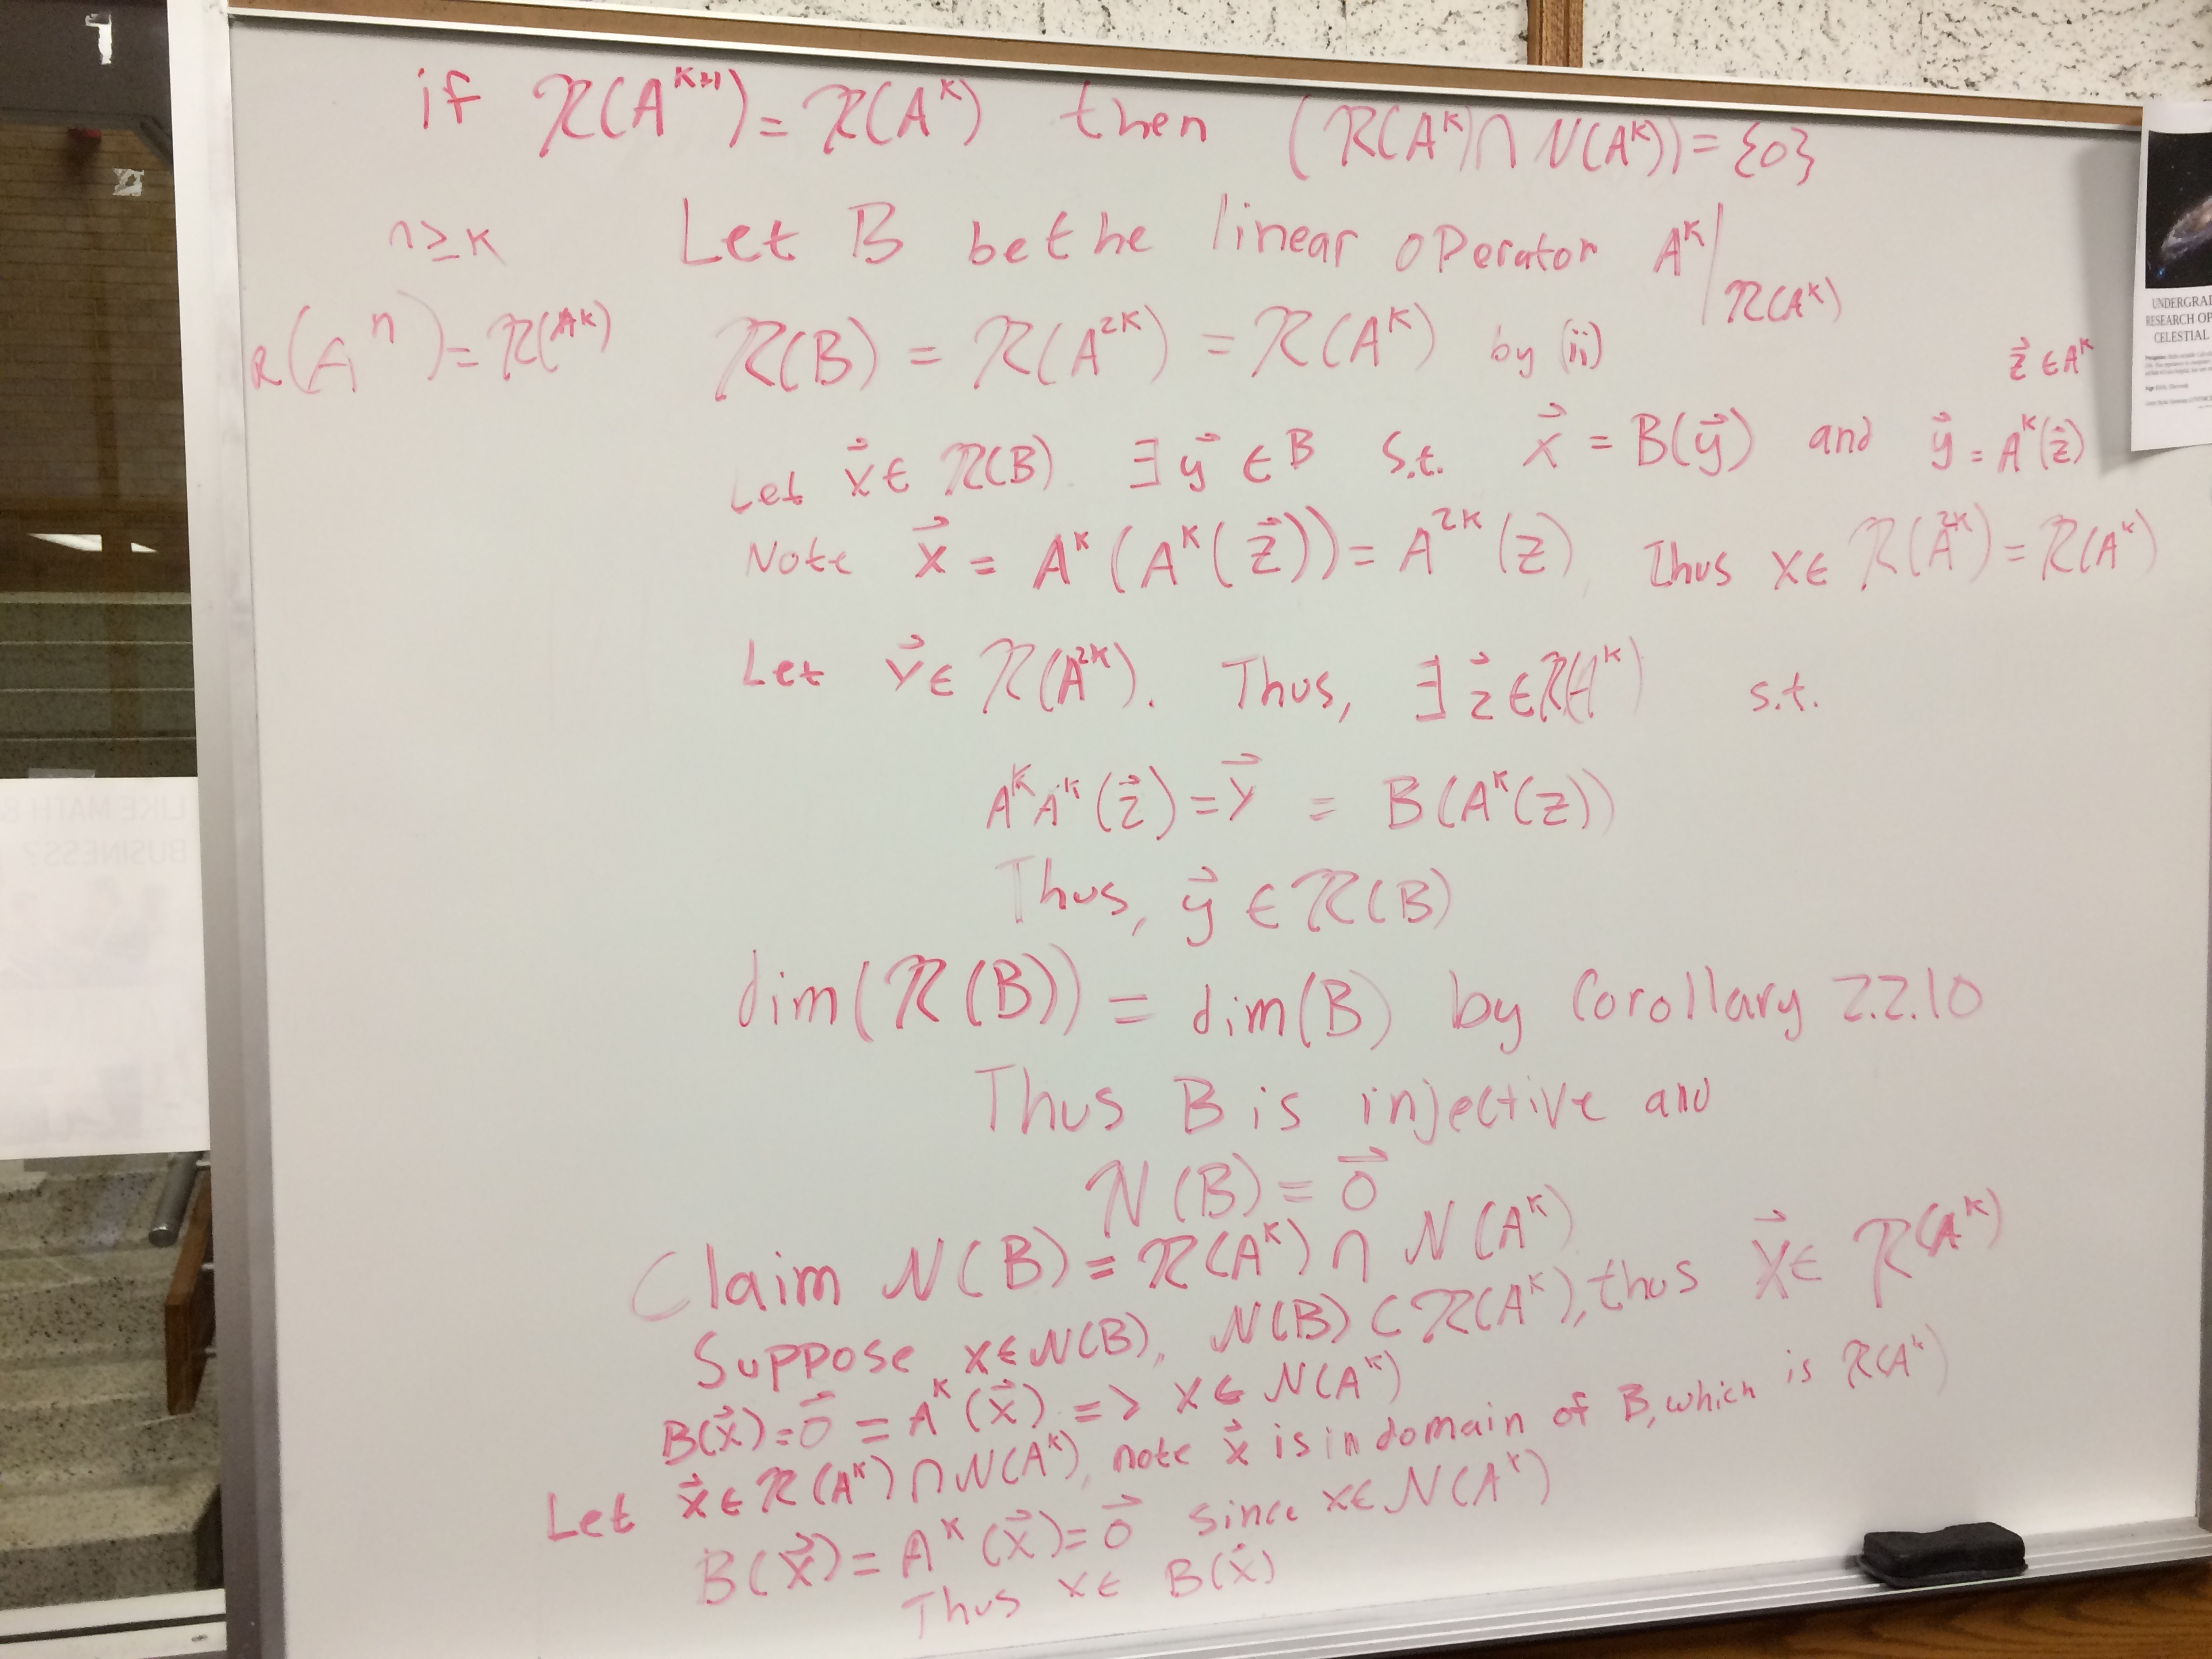
\includegraphics[scale=.1]{IMG_1297.JPG}

\subsection*{2.10}
Let $A': \mathscr{R} (B) \rightarrow W$
By the Rank-Nullity theorem, we have that $\text{dim} (\mathscr{R} (B))= \text{rank}(A') + \text{nullity} (A') \implies \text{rank} (B)= \text{rank}(A') + \text{nullity} (A')$.
Now we have to show that 
\[\mathscr{R}(A') = \mathscr{R} (AB) \quad \text{and that} \]
\[\mathscr{N}(A') = \mathscr{N} (A) \cap \mathscr{R} (B)\]
For the first equality, take an arbitrary $x \in \mathscr{R} (A')$. $x$ is mapped from $\mathscr{R} (B)$ to $W$. 
An arbitrary $y \in \mathscr{R} (AB)$ is mapped from $U\rightarrow \mathscr{R} (B) \rightarrow W \implies \mathscr{R} (A') =\mathscr{R} (AB)$
For the second equality, take an arbitrary $x \in \mathscr{N} (A'), y \in \mathscr{N} (A) \cap \mathscr{R} (B)$. The $\mathscr{N} A'$ is everything that is in the range of B but mapped to zero. The second term is every $y \text{ s.t. } B(y) = 0 y \in V$ that is mapped to zero but is also in $V$. Therefore, it is clear that
\[\mathscr{R}(A') = \mathscr{R} (AB)  \]
\[\mathscr{N}(A') = \mathscr{N} (A) \cap \mathscr{R} (B)\]



\subsection*{2.11 (i)}
\begin{align*}
    \text{Need to show rank} (AB) \leq \text{rank} A \text{and} rank(AB) \leq \text{rank} (B).  
\end{align*}
We know that $\text{rank} (AB) = \text{rank} B - \text{dim} (\mathscr{N} (A) \cap \mathscr{R} (B))$.
$\text{dim} (\mathscr{N} (A) \cap \mathscr{R} (B))$ cannot be negative, so we know that $\text{rank} (AB) \leq \text{rank} B$.
As for $\text{rank} (A)$, we know that 
\[\text{rank} (AB) = \text{rank} (B) - \text{dim} (\mathscr{N} (A) \cap \mathscr{R} (B)) \leq \text{rank} (A)\]
\[\implies \text{rank} (B) \leq \text{dim} (\mathscr{N} (A) \cap \mathscr{R} (B)) + \text{rank} (A)\]
Case one: $\text{dim} \mathscr{N} (A) > \text{dim} \mathscr{R} (B): \text{dim} (\mathscr{N} (A) \cap \mathscr{R} (B)) \leq \text{dim} \mathscr{R} (B) = \text{rank} (B)$ so we have that
\[ \text{rank} (B) \leq \text{rank} (A) + \text{rank} (B) \text{ if and only if } 0 \leq \text{rank} (A)\]
Case two: $\text{dim} (\mathscr{N} (A) \cap \mathscr{R} (B)) \leq \text{dim} \mathscr{N} (A)$,
so \[\text{rank} (B) \leq \text{rank} (A) + \text{nullity} (A) = \text{dim} (A) \text{by rank nullity} \]
\[\mathscr{R} (B) \subset V \implies \text{rank} B \leq \text{dim} V \implies \text{rank} (AB) \leq  \text{rank} (A)\]

\subsection*{2.11 (ii)}

We want to show that
\begin{align*}
    \text{rank} (A) + \text{rank} (B) - \text{dim} V \leq \text{rank} (AB)
\end{align*}

Note that

\begin{align*}
    \text{rank} (A) + \text{rank} (B) - \text{nullity} A - \text{rank} A = \text{rank} B - \text{dim} \mathscr{N} (A) \leq \text{rank} (AB) \\
    \implies \text{rank} B - \text{dim} \mathscr{N} (A) \leq \text{rank} B - \text{dim} (\mathscr{N} (A) \cap \mathscr{R} (B))\\
    \implies -\text{dim} \mathscr{N} (A) \leq  - \text{dim} (\mathscr{N} (A) \cap \mathscr{R} (B))\\
    \implies \text{dim} \mathscr{N} (A) \leq   \text{dim} (\mathscr{N} (A) \cap \mathscr{R} (B))\\
    \text{which is true } \implies \text{rank} (A) + \text{rank} (B) - \text{dim} V \leq \text{rank} (AB)\\
\end{align*}

\subsection*{2.12}
For the mapping $L$, and $a,b \in \mathbb{R}, ~ x,y \in V$ we have the following: \\ \\
\begin{align*}
L(ax + by) &= \Big( (ax+by) + W_1, (ax+by) + W_2,\dots, (ax+by) + W_n \Big) \\
aL(x) + bL(y) &= a\Big(x+W_1, x+W_2,\dots, x+W_n \Big) + b\Big(y+W_1, y+W_2,\dots, y+W_n \Big)\\
&= \Big(ax+W_1, ax+W_2,\dots, ax+W_n \Big) + \Big(by+W_1, by+W_2,\dots, by+W_n \Big) \\
&= \Big( (ax+by) + W_1, (ax+by) + W_2,\dots, (ax+by) + W_n \Big) \\
\end{align*}
$\implies L$ is a linear transformation. \\ \\
To show that $\mathscr{N}(L) = \cap_{i=1}^n W_i$, we notice that: 
\begin{align*}
\mathscr{N}(L) &= \{x \in V ~|~ x + W_i = 0 + W_i~ \forall~i\} = \{x \in V ~|~ x \in W_i~\forall~i\} \\
&= W_1 \cap W_2 \cap \dots \cap W_n = \cap_{i=1}^n W_i \\
\end{align*}

\subsection*{2.13}
If $V$ is a vector space and $S \subset T \subset V$, and $L: V/S \rightarrow V/T$ such
that \\$
L(x+S)=(x+T)$. \\ \\
We know that the mapping $L$ is well defined because $S \subset T$ and for any 
$(x + T)\in V/T$ the mapping is given by $(x+T)\in V/S$. This allows us to say that
the mapping $L$ is surjective. \\
\\
We now want to show that our mapping $L$ is linear:
\begin{align*}
    \mathscr{N}(L) &= \{ (x + S) \in V/S ~|~ L(x+S)=(x+T)\} \\
    &= \{ (x+S) \in V/S ~|~ x \in T \} \\
    &= \{ x+S \in T/S\}
\end{align*}
$\implies L$ is linear and by the FIT we have
$\frac{V/S}{T/S}$ is isomorphic to $V/T$.

\end{document}
